\chapter{Data Analysis}

\section{Dredging activity}
This section describes the relevance of dredging to the sediment balance of the designated area, by an estimation of the dredging volumes through different data sources. 


\subsection{Vessel positioning information (AIS)}
The number of vessels engaged in dredging activities on the Paraná Guazú was determined using AIS (Automatic Identification System) data. Vessel movements between dredging sites and ports were monitored through \textit{MarineTraffic}. Although historical records were not considered, the daily activity observed during the study period provides a reliable estimate of the sand extraction volumes.


\subsection{Extraction permits}
To avoid adverse impacts on the hydraulic regime from dredging, companies must first obtain permits from the \textit{National Water Institute }(INA). These permits specify the locations and volumes of the proposed dredging activities. The information they provide serves as a reliable estimate of the total material being removed from the river, thereby influencing the sediment balance. Therefore, the permits were analysed for the area of interest.

A total of 33 permits were collected for the Paraná Guazú and 43 for the Ibicuy. On the Paraná Guazú, four permits were issued for channel maintenance, while the remainder concerned sand extraction. For the Ibicuy, all permits were related to extraction activities. The analysis shows that the requested volumes in the Ibicuy are considerably larger than those in the Paraná Guazú, even though the section of the Ibicuy considered here is much shorter in length.

It is important to note that the end dates of contracts are unknown. While the requests specify monthly dredging quantities, they do not indicate the duration of the works. As a result, a detailed quantitative assessment cannot be made. For the present analysis, all requests with fixed monthly volumes are assumed to extend over 12 months, allowing for a comparison between the two river sections, as shown in Figure \ref{fig:yearly dredging volumes}. The second assumption is to record a single value for the requested volume, when information about monthly or yearly occurrence is lacking.

\begin{figure}[H]
    \centering
    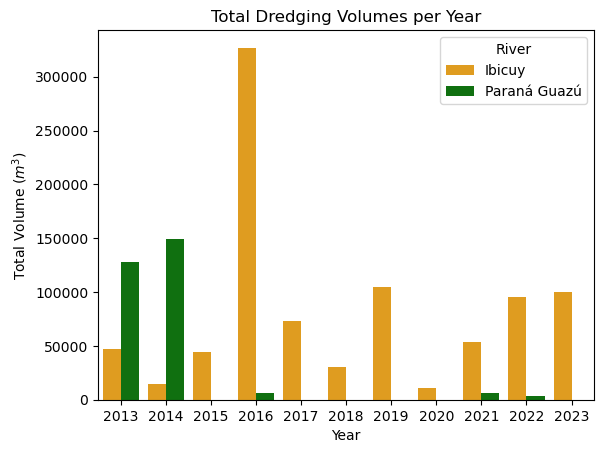
\includegraphics[width=0.75\linewidth]{figures/figure chap 2/Dredging volumes permits.png}
    \caption{Yearly dredging volumes}
    \label{fig:yearly dredging volumes}
\end{figure}

\subsection{Estimated sand extraction}

\section{Hydrodynamic data}
\section{Sediment transport}

% \section{Water Quality and Bioorganism Activity?}

